\documentclass[tikz,crop]{standalone}

\usepackage{tikz}
\usetikzlibrary{calc, positioning, fit}

\begin{document}
    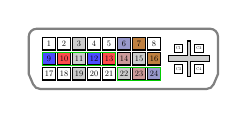
\begin{tikzpicture}[
        outline/.style = {%
            thick,%
            draw=black!50,%
        },%
        digital pin/.style = {%
            draw,%
            rectangle,%
            minimum size=1.6mm*2.5*4/3,%
            inner sep=0pt,%
            scale=0.3% to scale the font
        },%
        analog pin/.style = {%
            draw,%
            rectangle,minimum size=1.1mm/0.15,%
            inner sep=0pt,%
            scale=0.15% to scale the font
        },%
        gnd pin/.style = {%
            fill=white!50!black!40%
        },%
        positive pin/.style = {%
            fill=red!50!black!40%
        },%
        negative pin/.style = {%
            fill=blue!50!black!40%
        },%
        anode pin/.style = {%
            fill=red!70%
        },%
        cathode pin/.style = {%
            fill=blue!70%
        },%
        io pin/.style = {%
            fill=brown%
        },%
        shield/.style = {%
            draw,%
            line width=0.1mm,%
            inner sep=0.1pt,%
            green!80!black,%
        },%
    ]
        \begin{scope}[shift={(-12.015mm, -3.75mm)}]
        % Outline
        \draw[outline]
            (0,0) arc(270:203:1mm) -- ++(113:1.4mm) -- ++(0,4.75mm) arc(180:90:1mm) -- ++(22.03mm,0) arc(90:0:1mm) -- ++(0,-4.75mm) --++(247:1.4mm) arc(-23:-90:1mm) -- cycle
        ;
        % Digital pins
        \tikzset{fillpins/.code={%
            \ifnum #1=3 \tikzset{gnd pin}\else%
            \ifnum #1=6 \tikzset{negative pin}\else%
            \ifnum #1=7 \tikzset{io pin}\else%
            \ifnum #1=9 \tikzset{cathode pin}\else%
            \ifnum #1=10 \tikzset{anode pin}\else%
            \ifnum #1=11 \tikzset{gnd pin}\else%
            \ifnum #1=12 \tikzset{cathode pin}\else%
            \ifnum #1=13 \tikzset{anode pin}\else%
            \ifnum #1=14 \tikzset{positive pin}\else%
            \ifnum #1=15 \tikzset{gnd pin}\else%
            \ifnum #1=16 \tikzset{io pin}\else%
            \ifnum #1=19 \tikzset{gnd pin}\else%
            \ifnum #1=22 \tikzset{gnd pin}\else%
            \ifnum #1=23 \tikzset{positive pin}\else%
            \ifnum #1=24 \tikzset{negative pin}\else%
            \fi\fi\fi\fi\fi\fi\fi\fi\fi\fi\fi\fi\fi\fi\fi%
        }}
        \foreach \j in {0,...,2} {
            \foreach[evaluate={\n=int(\j*8+\i+1)}] \i in {0,...,7} {
                \node[digital pin,fillpins=\n] (pin\n) at (\i*1.905mm+1.105mm,\j*-1.905mm+5.75mm){\n};
            }
        }
        % Analog pins
        \node[analog pin] at (17.55mm,5.15mm)(C1){C1};
        \node[analog pin] at (20.15mm,5.15mm){C2};
        \node[analog pin] at (17.55mm,2.55mm){C3};
        \node[analog pin] at (20.15mm,2.55mm)(C4){C4};
        \draw[gnd pin]
            ($(C1)!0.5!(C4)$) ++(-2.62mm,0.35mm) -- ++(2.42mm,0) -- ++(0,1.9mm) -- ++(0.4mm,0) -- ++(0,-1.9mm) -- ++(2.42mm,0) -- ++(0,-0.7mm) -- ++(-2.42mm,0) -- ++(0,-1.9mm) -- ++(-0.4mm,0) -- ++(0,1.9mm) -- ++(-2.42mm,0) --cycle
        ;
        % Shields
        %\node[shield, fit={(pin1) (pin2) (pin3)}]{};
        \node[shield, fit={(pin9) (pin10) (pin11) (pin12) (pin13)}]{};
        %\node[shield, fit={(pin17) (pin18) (pin19)}]{};
        \node[shield, fit={(pin22) (pin23) (pin24)}]{};
        \end{scope}
        % Grid
        %\draw[step=1cm,gray,very thin] (-6,-3) grid (0,0);
    \end{tikzpicture}
\end{document}
